%!TEX root = ../Thesis.tex

\chapter{工作总结与展望}\label{chapter:conclusion}

从卷积神经网络在 2012 年的兴起~\cite{Krizhevsky2012ImageNetCW} 到图像检索领域的研究者将卷积神经网络与图像检索的技术结合起来~\cite{Babenko2014NeuralCF,Gong2014MultiscaleOP} ,再到最近基于卷积神经网络的方法在常用的一些数据库上效果已经超过了传统的方法~\cite{Gordo2016DeepIR,Noh2017LargeScaleIR},短短四五年时间,基于卷积神经网络的方法在图像检索方向就取得了巨大的进步。本文的工作也是围绕卷积神经网络在图像检索领域的应用展开的,同时结合了对与敏感枪支图像检索的需求,下面对本文的的工作做一总结,并对未来工作进行展望。

\section{工作总结}
本文围绕卷积神经网络在图像检索领域的应用,分析了目前方法的优缺点,并且结合对敏感图像识别的需求,开展了相关的工作,主要工作总结如下:

\begin{enumerate}
\item 我们建立了一个大规模的枪支图像数据库

在社交网络上,大量的枪支图片会引起用户不适,需要适当的控制与处理。目前的基于深度卷积神经网络的检索方法,在模型的训练过程中都需要大量的训练数据,否则模型将过拟合。这些都要求一个数据量丰富的数据库,从而方便研究者开展该方面的研究,但是目前并没有一个大规模的枪支图片数据库存在。为了这样的需求,我们构建了一个大规模的枪支图像数据库,该数据包含 14755 张来自 167 类不同类型枪支的图片,可以为枪支图片分类与检索研究提供所需的数据基础。

\item  我们提出了一种多尺度全卷积的图像实例检索方法

在工作中,我们发现目前基于卷积神经网络的图像检索方法在提取图像特征时,并未详细分析影响提取的特征有效性的因素,采用的设置都是一些比较随意的选择,因此我们通过实验详细分析了三个重要因素对提取的特征有效性的影响,这三个因素分别是:输入神经网络的图像尺寸,多尺度特征表达以及 PCA 和白化矩阵的学习方式。结合我们的实验和分析,我们提出了一种多尺度全卷积的图像实例检索方法,我们的方法在多个数据库上都取得了良好的效果。

\item 我们提出了一种基于双阈值对比损失函数的枪支图像检索方法

在当前的社交网络上,大量的枪支图片的出现,要求社交媒体的监管者对这些图片进行适当的处理,在取证中,也有大量需要鉴定枪支图片类型的需求,这些问题都可以通过图像检索相关的技术得到有效解决。在本工作中,我们研究了微调卷积神经网络进行枪支图片检索的可行性,我们发现,传统的单阈值对比损失函数对于枪支图像检索,存在一定的缺点:第一,使用该函数,在模型的训练过程中,正负样本贡献的损失不平衡,模型的训练偏向负样本对;第二,由于枪支图片与训练这些基础模型的 ImageNet 存在巨大的域差异,直接使用这些模型针对检索任务微调,并不能取得良好的效果。我们提出使用双阈值对比损失函数解决网络训练中正负样本贡献的损失不平衡的问题。我们采用两步训练的策略缓和域差异带来的性能下降问题,第一步,我们在 Firearm14k 上针对分类任务微调网络,第二步再针对检索任务(使用双阈值对比损失函数)微调模型。在 Firearm14k 测试集上,我们把提出的方法与其他主流方法进行了对比,实验结果表明,我们的方法得到的检索结果在不同特征维度上都要优于其他的方法。
\end{enumerate}

\begin{figure}
\centering
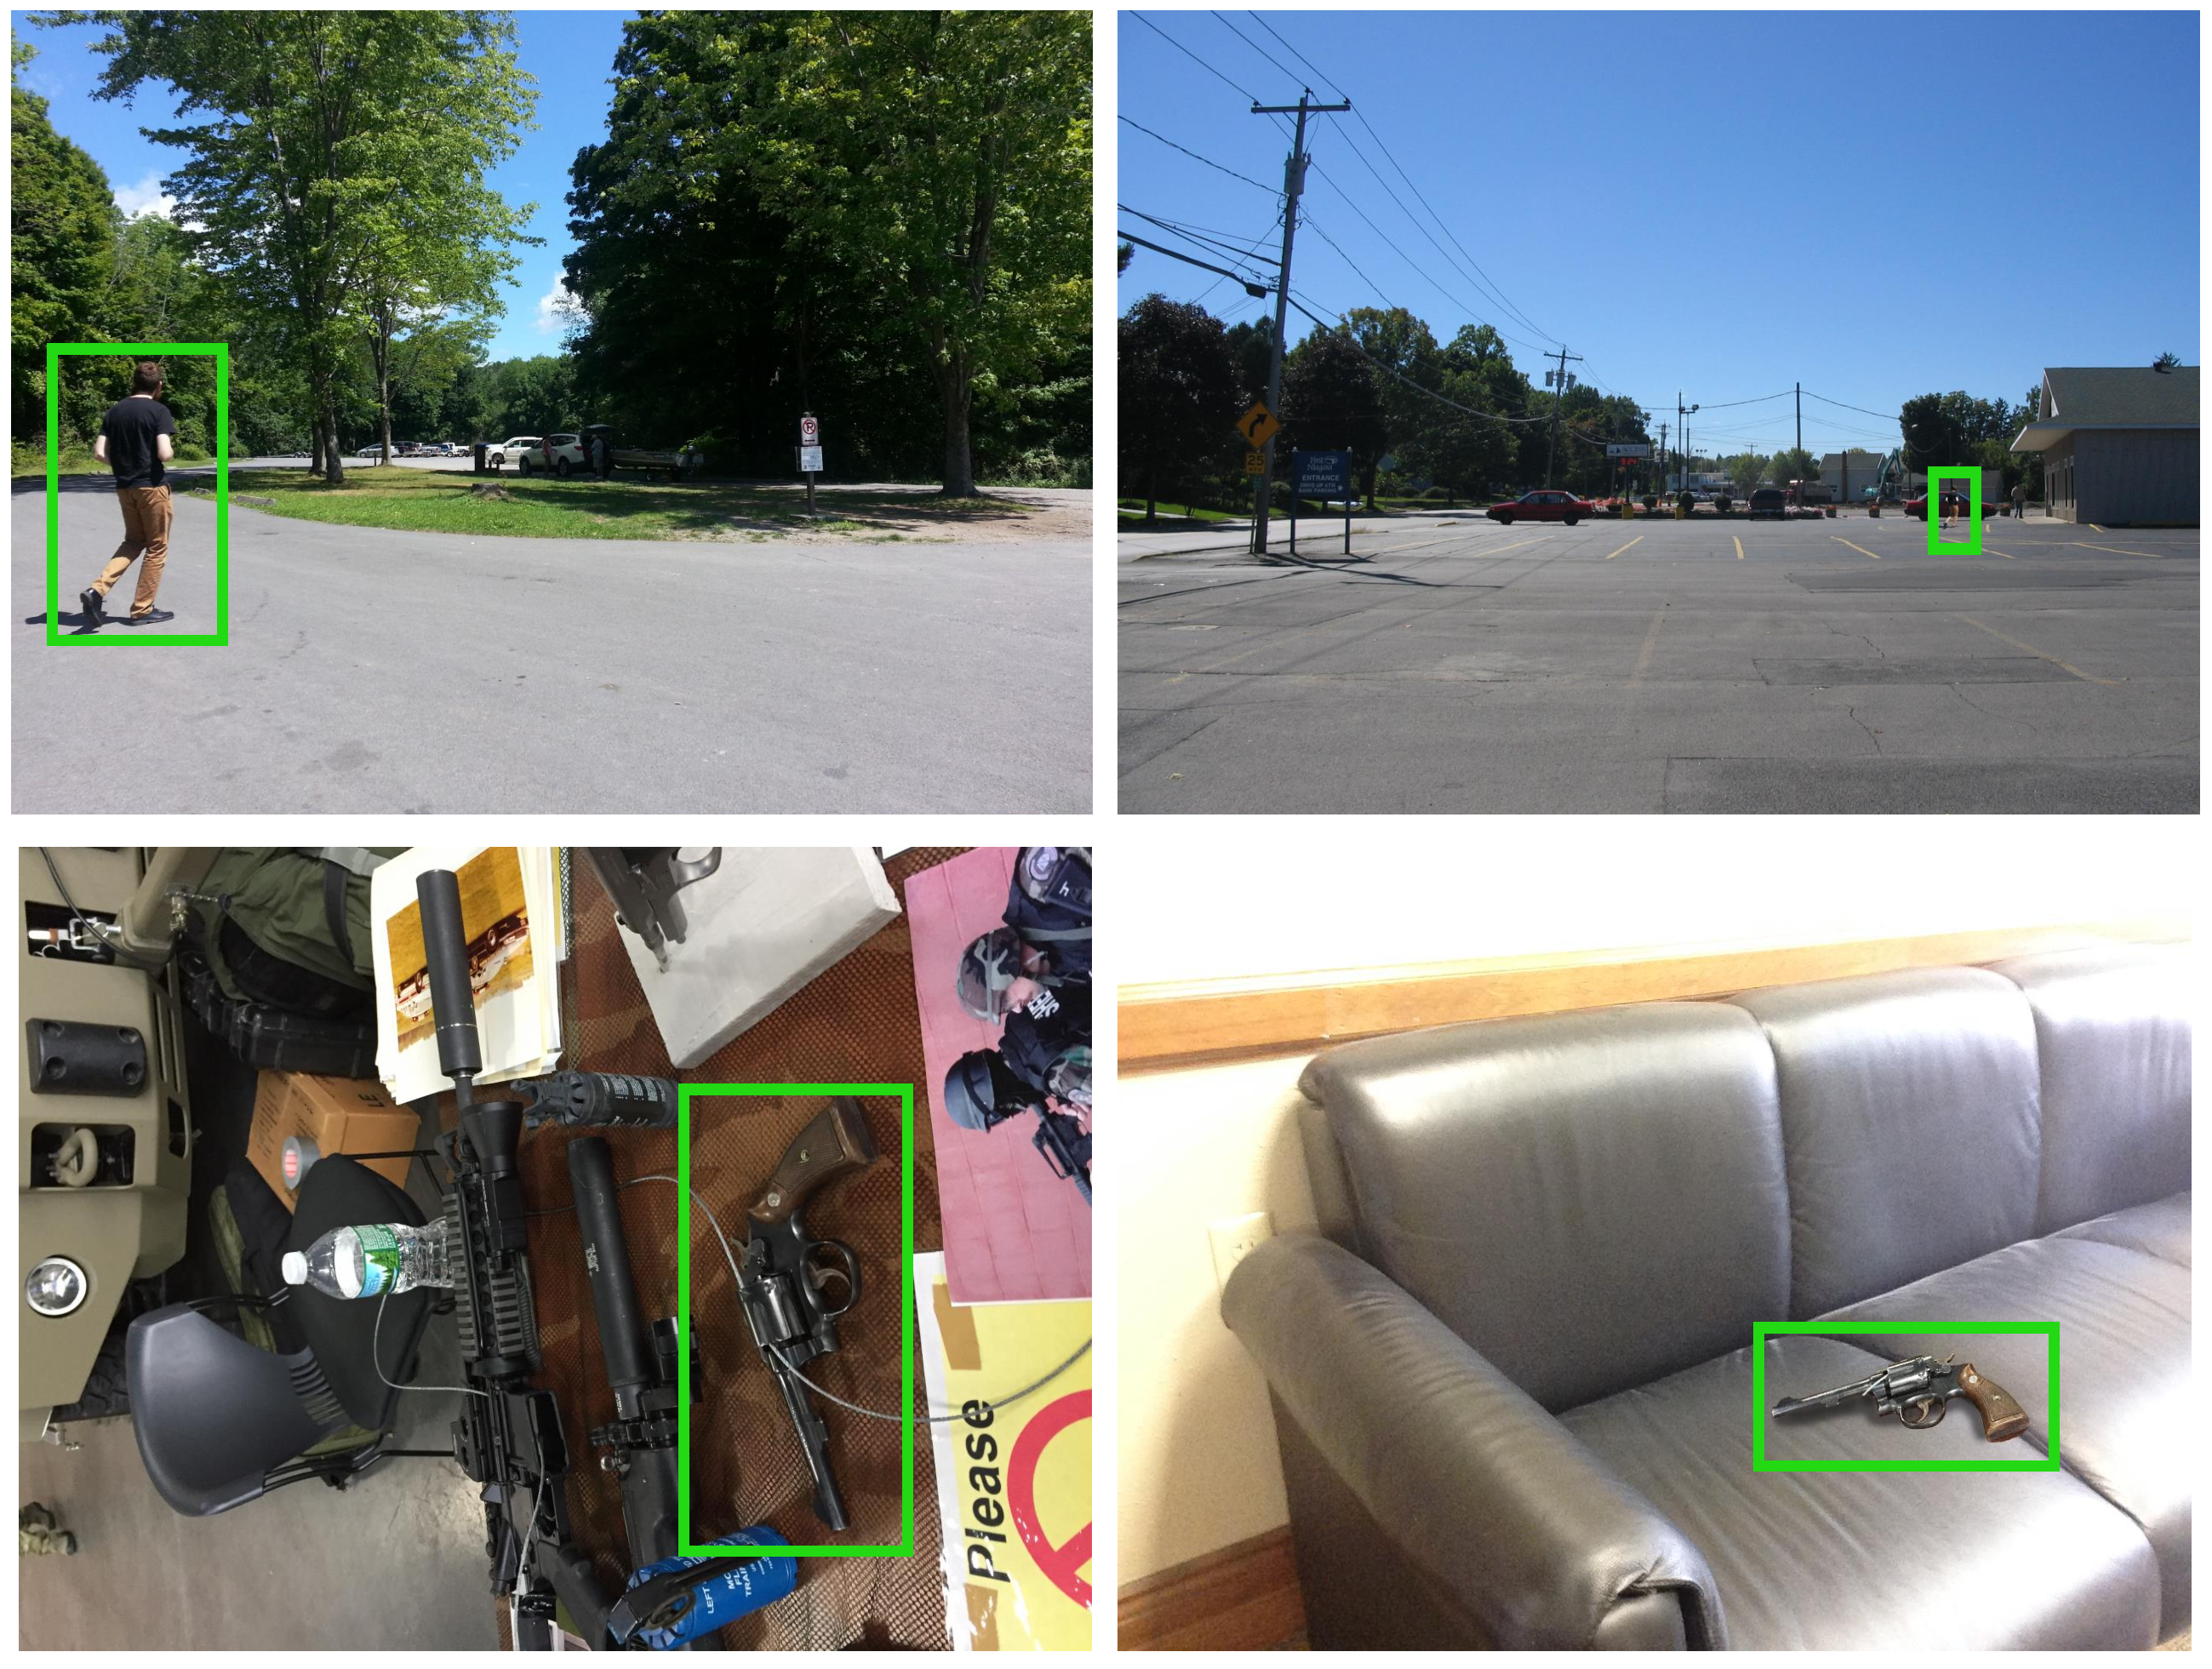
\includegraphics[width=\columnwidth]{chapter_conclusion_forensic_retrieval.pdf}
\caption[两个图片剪切篡改的实例]{两个图片剪切篡改的实例(\textbf{左}:donor 图片,\textbf{右}:剪切拼接后图片),请放大查看}
\label{fig:forensic_image_retrieval}
\end{figure}

\section{工作展望}
虽然我们的方法在图像检索任务上取得了不错的结果,但是该领域仍有许多没有完全解决的问题,未来的工作将关注以下几个问题:

\begin{enumerate}
\item 利用显著性分析或注意力机制解决图像中小物体检索的问题

在我们的工作中,我们发现基于卷积神经网络的方法,在图像中的物体尺寸非常小的情况下,效果并不理想,因为卷积神经网络提取的是图像的全局特征,并不像 SIFT 特征描述子一样提取的是局部特征。包含小物体的图像,如果使用卷积神经网络提取特征,特征中可能包含了大量周边环境的特征,对小物体的检索造成了干扰,我们可以结合一些显著性分析或者注意力机制的方法~\cite{Song2017DeepSA},自动检测图像中可能的物体,然后提取显著性区域的特征,忽略周边环境的干扰,从而增强小物体图像检索的有效性。

\item 研究基于深度学习的局部特征描述特征

深度学习特征本质上是图像全局信息的表达,特别是网络经过多层卷积与池化以后,特征图一个元素在原图上对应着很大一片区域(感受野比较大),无法像传统的 SIFT 特征一样,进行空间几何校验,进行检索结果重排序,提高检索的准确率度。目前这方面的工作还比较少,Noh 等~\cite{Noh2017LargeScaleIR} 提出的方法就是试图学习局部深度特征,但是他们使用的训练方法并未针对检索的任务,局部特征有效性有待提高,因此这方面的研究也是未来的一个方向。

\item 研究基于特征量化和哈希的精细图像检索问题

在本文中所使用的特征都是实值特征,并不是二值化的特征,在检索数据库规模小的情况下,这些方法是可行的,但是当数据库规模巨大(亿级别或者十亿级别)时,这样的方法弊端是明显的,一方面特征存储需要消耗大量空间,另外计算特征之间的相似度也会消耗大量时间,达不到实时性的要求。另外目前哈希方法使用的数据库都是一些粗糙类别层次的数据库,如 CIFAR10\footnote{\url{https://www.cs.toronto.edu/~kriz/cifar.html}},NUSWIDE~\cite{Chua2009NUSWIDEAR},并不是精细类别的数据库,因此基于特征量化或者深度学习的图像特征哈希编码学习也是一个非常重要的研究方向。

\item 利用图像检索的方法解决图像取证的问题

随着数字图像技术的发展,图像伪造技术也不断进步,网络上以及媒体上出现了各种伪造的照片。在图像取证中,有一类图片伪造方法是剪切拼接(splicing)~\cite{Farid2009ImageFD},也就是把一张图片(称为 donor 图片)一部分剪切拼接到另一张图片上(称为 base 图片),达到欺骗目的,图~\ref{fig:forensic_image_retrieval} 展示了两例剪切拼接的实例(绿色框中是对应的相同物体)。如果能通过搜索技术找到剪切后的图像中物体的原图,那么就可以很容易判断图像是被篡改过的,因此基于图像检索的技术也能在剪切检测中发挥一定的作用。
\end{enumerate}







